\documentclass[a4paper,12pt]{article}

\title{Physics 30 \\ Electromagnetic Radiation - Optics}
\author{Jad Chehimi}

% document setup
\renewcommand{\familydefault}{\sfdefault}
\linespread{1.25}
\usepackage[margin=1in]{geometry}
\usepackage{setspace}
\usepackage{enumitem}
\setlist{nosep}
\usepackage{color,soul}
\setcounter{secnumdepth}{0}

% tools
\usepackage[hidelinks]{hyperref}
\usepackage{float}
%% images
\usepackage{graphicx}
\graphicspath{ {./images/} }
%% science
\usepackage{siunitx}
\sisetup{exponent-product=\times, per-mode=fraction}

\begin{document}
\maketitle

% temp
\begin{center}
\Huge
Unfinished!
\normalsize
\end{center}
% temp

\tableofcontents

\pagebreak

\section{Electromagnetic Spectrum}
\begin{figure}[H]
    \centering
    \caption{"Cosmic" rays on the left of gamma}
    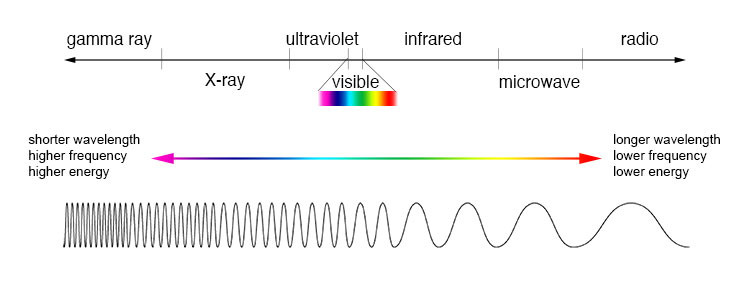
\includegraphics[width=\textwidth]{emr}
\end{figure}
\begin{itemize}
    \item{ALL EMR travels at the speed of light. ($c = \SI{3.00e8}{\m\per\s}$)}
    \item{
        \hl{Memorize the visible spectrum wavelength range}
        \begin{itemize}
            \item{\SI{400}{\nano\m} to \SI{750}{\nano\m}}
            \item{\SI{400e-9}{\m} to \SI{750e-9}{\m}}
        \end{itemize}
    }
\end{itemize}

\subsection{Universal Wave Equation}
\Large $$v = f\lambda$$ \normalsize
\begin{itemize}
    \item{$v$ = speed (\si{\m\per\s})}
    \item{$f$ = frequency (\si{\Hz})}
    \item{$\lambda$ = wavelength (\si{\m}) (often given in nanometers, $\SI{100}{\nano\m} = \SI{100e-9}{\m}$)}
\end{itemize}

Speed of light: $c = f\lambda$

\subsection{Transverse Wave}
\begin{figure}[H]
    \centering
    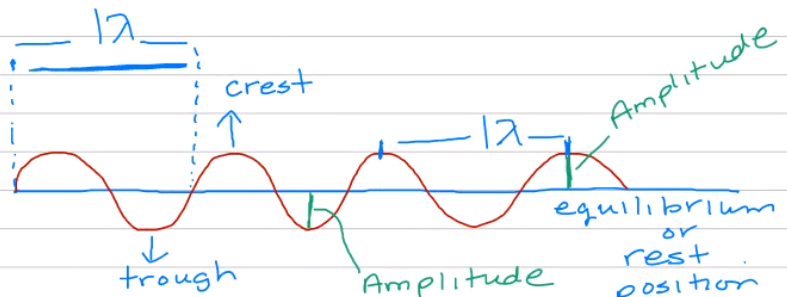
\includegraphics[width=0.9\textwidth]{transverse}
\end{figure}
\begin{itemize}
    \item{\textbf{Crest}: peak of wave}
    \item{\textbf{Trough}: depression of wave}
    \item{\textbf{Amplitude}: the maximum displacement from the equilibrium position}
\end{itemize}

\section{Law of Reflection}

\Large $$\angle{I} = \angle{R}$$ \normalsize

\begin{figure}[H]
    \centering
    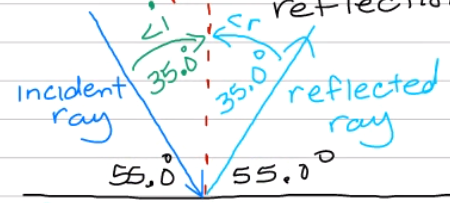
\includegraphics[width=0.50\textwidth]{reflect}
\end{figure}

\begin{itemize}
    \item{$\angle{I}$: \textbf{Angle of Incidence} \\Measured from the light ray to the normal}
    \item{$\angle{R}$: \textbf{Angle of Reflection} \\Measured from reflected ray to normal}
    \item{
            \textbf{Normal}
            \begin{itemize}
                \item{Perpendicular to the surface}
                \item{Broken/dotted line}
                \item{Drawn from where the incident ray contacts the mirror surface}
            \end{itemize}
        }
\end{itemize}

\subsection{Example}
A light ray strikes a flat mirror at an angle of \ang{70.0} to the mirror surface. What is the angle of reflection? What is the angle between the incident ray and the reflected ray?
\begin{figure}[H]
    \centering
    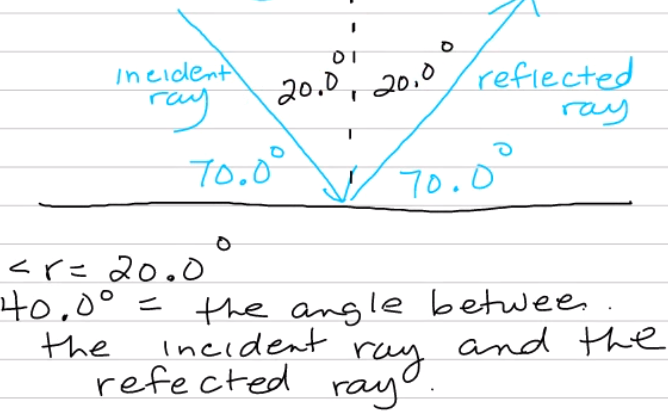
\includegraphics[width=0.6\textwidth]{ex-reflect}
\end{figure}

\section{Refraction}
The bending of a wave when entering a new medium at an angle.

\begin{itemize}
    \item{$n$: Index of Refraction (air is $n = \num{1.00}$)}
    \item{When a light ray travels from a lower $n$-value medium to a greater $n$-value medium, the light ray will \hl{bend toward the normal}}
\end{itemize}

\subsection{Snell's Law}
\Large $$n_1\sin{\theta_1} = n_2\sin{\theta_2}$$ \normalsize
Use to calculate the new angle in a different medium/n value.

\Large $$\frac{n_2}{n_1} = \frac{\sin{\theta_1}}{\sin{\theta_2}} = \frac{\lambda_1}{\lambda_2} = \frac{v_1}{v_2}$$ \normalsize

\subsection{Frequency}
Frequency is \hl{unaffected by medium}. 

Frequency can only be changed at the source.

\subsection{Critical Angle}
Two conditions must be met for a critical angle.
\begin{itemize}
    \item{The light must travel from a \hl{greater $n$-value to a lesser $n$-value}}
    \item{The angle of refraction must be \ang{90.0}}
\end{itemize}
\begin{figure}[H]
    \centering
    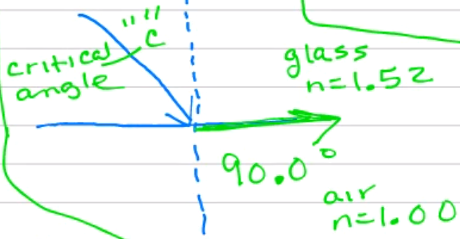
\includegraphics[width=0.50\textwidth]{criticalangle}
\end{figure}

\subsection{Total Internal Reflection}
If the angle of incidence is \hl{greater than the critical value}, then the ray will \hl{reflect instead of refract}.

Trying to calculate this angle with Snell's Law will error.

\subsection{Examples}
\subsubsection{Parallelogram}
\begin{figure}[H]
    \centering
    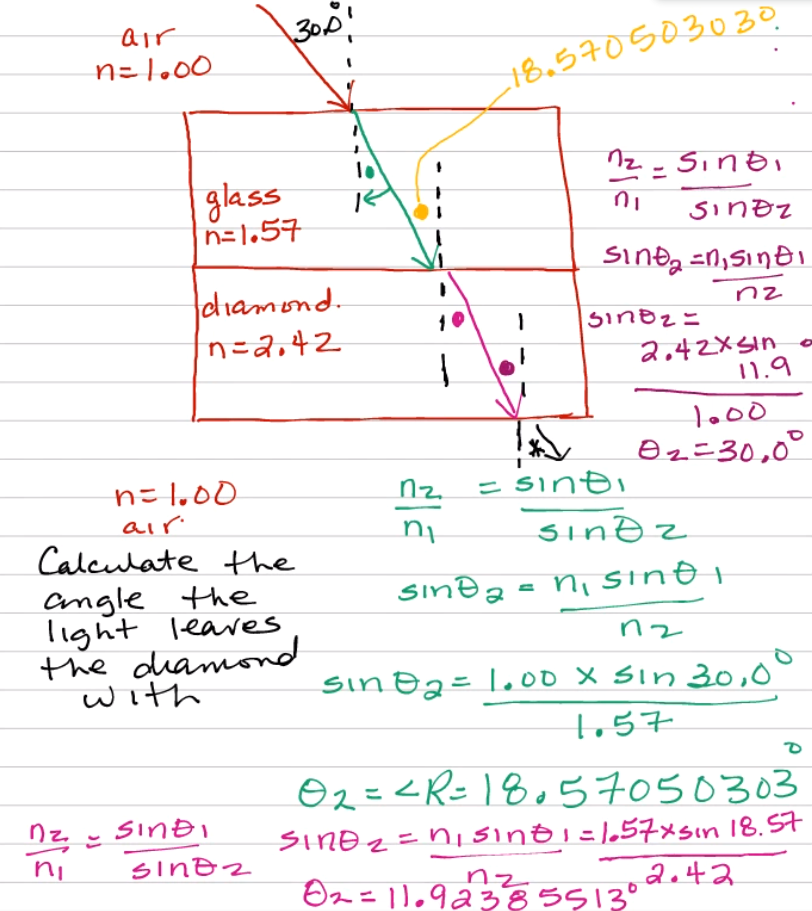
\includegraphics[width=\textwidth]{ex-sqr}
\end{figure}

\subsubsection{Equilateral Triangle}
\begin{figure}[H]
    \centering
    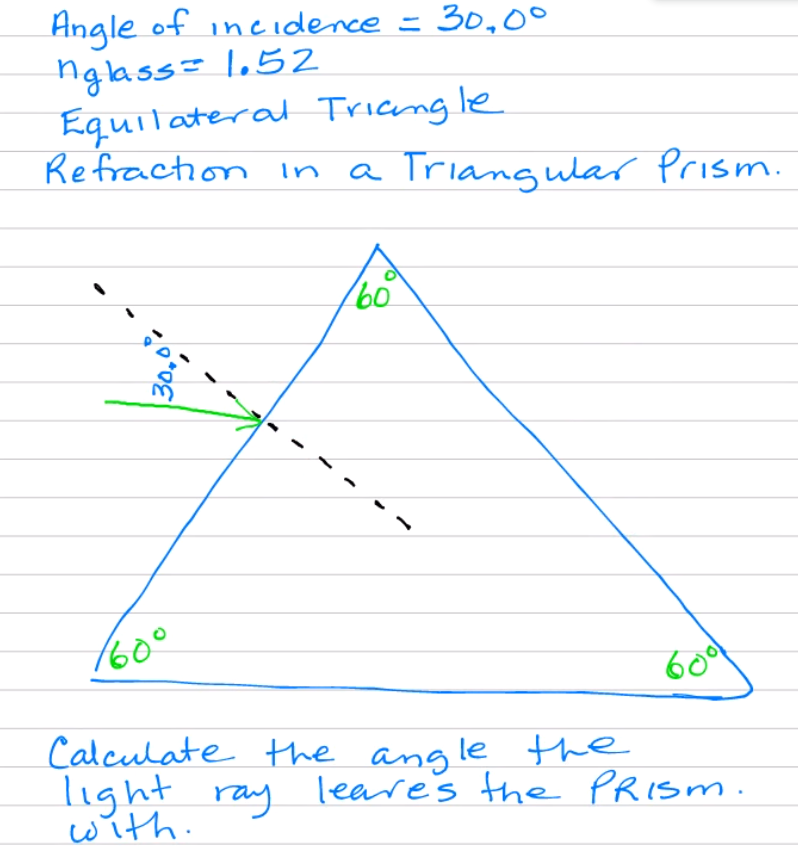
\includegraphics[width=0.45\textwidth]{ex-tri-1}
    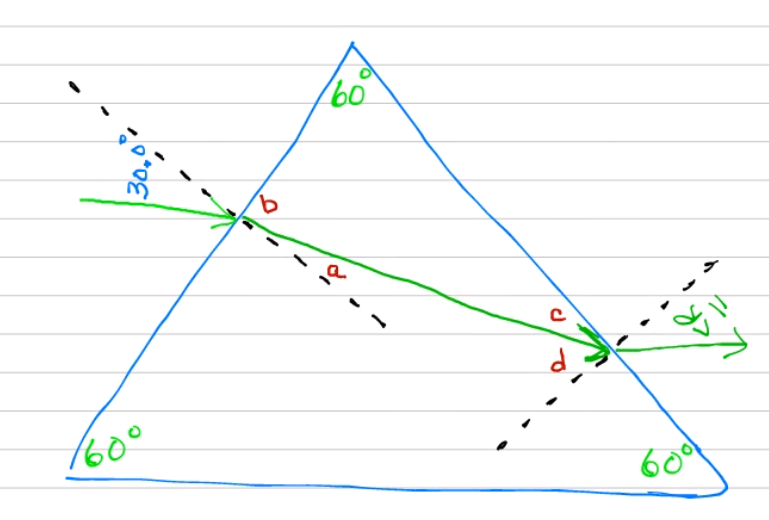
\includegraphics[width=0.45\textwidth]{ex-tri-2}
\end{figure}
\begin{figure}[H]
    \centering
    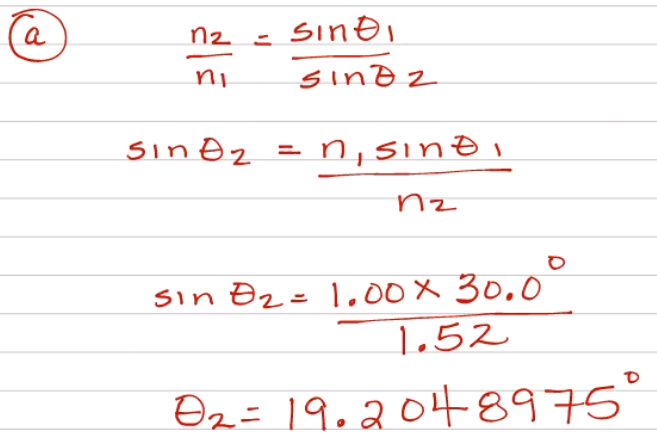
\includegraphics[width=0.45\textwidth]{ex-tri-3}
    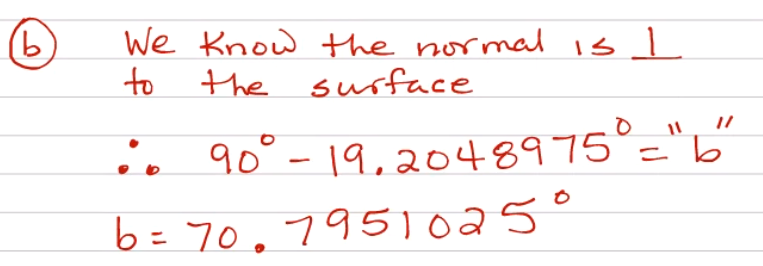
\includegraphics[width=0.45\textwidth]{ex-tri-4}
\end{figure}
\begin{figure}[H]
    \centering
    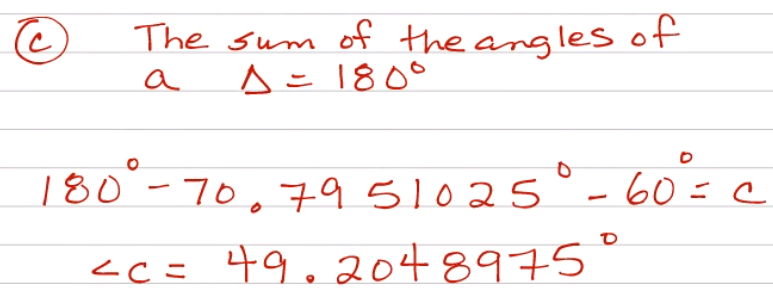
\includegraphics[width=0.45\textwidth]{ex-tri-5}
    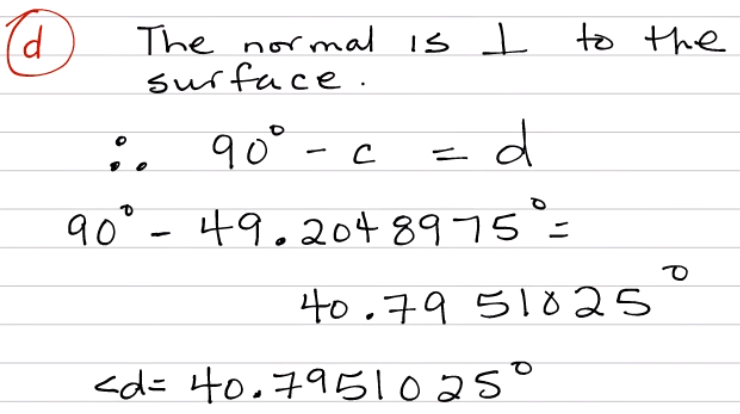
\includegraphics[width=0.45\textwidth]{ex-tri-6}
\end{figure}
$$\theta = \ang{83.3}$$

\end{document}
